\chapter{Evaluation p2p Overlay-Netzwerke}
\label{chap:evaluation_p2p}

Dieses Kapitel bietet einen Überblick über einige p2p-Netzwerke und evaluiert diese anhand gestellter Anforderungen. Diese Evaluation beeinflusst die Entscheidung für ein Overlay-Netzwerk, auf das schließlich das, in dieser Arbeit zu entwickelnde, generische Publish/Subscribe-System gesetzt wird. Die Evaluation bedient sich zahlreicher Arbeiten, die sich alleine dem Vergleich dieser Netzwerke widmen \cite{Lua2005Survey, Goetz2005, Li2004Comparing, Darlagiannis2006Peertopeer, Castro2002Secure, Bo2003PeertoPeer} und geht auch auf ihre Nutzbarkeit als Basis für \emph{Application level multicast} sprich ein Publish/Subscribe-System ein \cite{Hosseini2007Survey, Fahmy2007, Castro2003Evaluation, Ratnasamy2001}.

Zuvor müssen jedoch die eigenen Anforderungen an solche Systeme identifiziert werden. Zu den offensichtlichen Anforderungen wie beispielsweise \emph{Skalierbarkeit} gesellen sich jedoch auch spezielle Anforderungen aus Spielsicht hinzu. Diese sind beispielsweise das Vorhandensein eines dedizierten Servers zur Authentifizierung oder das Übertragen von Applikationswissen auf das Netzwerk um damit dessen Entscheidungen bezüglich Nachbarschaften oder Versand von Nachrichten (Routing) zu beeinflussen.

\section{Anforderungen an p2p-Netzwerke}

\paragraph{Geringe Latenz} Schnelle Reaktionszeiten und Nachrichtenübermittlung sind bei \ac{mmog} unverzichtbar. Ebenfalls müssen größere Nachrichten (beispielsweise Update der Welt) schnell übertragen werden, damit der Spielfluss nicht behindert wird. Dies lässt sich beispielsweise anhand der Anzahl der Hops beim Nachrichtenversand messen.

\paragraph{Skalierbar} Selbst bei einer großen Anzahl an Knoten soll das Netz nicht kollabieren. Hierbei ist es auch wichtig, dass Knoten nicht unbedingt lange im Spiel sein müssen. Zwar kann davon ausgegangen werden, dass ein durchschnittlicher Spieler längere Zeit im Spiel verbringt, aber durch Netzausfälle oder sonstigen Unbill kann dies stark variieren. Li untersucht in \cite{Li2004Comparing} wie sich p2p-Netzwerke bei großen Fluktuationen verhalten.

\paragraph{Fehlertoleranz bei Knotenausfall} Fallen Knoten aus, muss sich das Netz ohne großen Kommunikationsaufwand selbst reparieren. Auftretende Netzwerkpartitionierungen sind für diese Arbeit jedoch kein Hindernis, da durch den, über eine gesonderte Verbindung erreichbare, Authentifizierungsserver die notwendigen Informationen angefordert werden können um das Netz wieder zu verbinden.

Interessant hierbei ist auch die eingebaute Redundanz einiger Systeme, die Daten auf mehrere Knoten verteilen. Wie sich dies im Vergleich von statischen Daten zu sich häufig verändernden Objekten der Spielewelt verhält, ist zu untersuchen. 

\paragraph{Kommunikation über das Netzwerk} Das Netzwerk soll nicht nur das schnelle Auffinden von Peers ermöglichen, sondern auch einen Transport der Nachricht (Routing) durch das Netzwerk selbst bereitstellen.

\paragraph{Bestimmung der Nachbarschaft} Eine dynamische Bestimmung der Nachbarschaftsgröße kann von Vorteil sein. So könnten Knoten mit mehr Bandbreite (beziehungsweise entsprechenden anderen Metriken) mehr direkte Verbindungen halten als Knoten mit geringer Bandbreite (oder geringer Spieldauer).

\paragraph{Eingriff in Routingentscheidungen} Applikationswissen hilft auch beim Eingriff in das Routing des Netzes. So können Knoten bevorzugt zur Weiterleitung einer Nachricht ausgewählt werden. Diese Knoten zeichnen sich beispielsweise durch eine große Bandbreite oder spezielle Applikationsmetriken\footnote{Bsp: Spieler befindet sich in der selben Stadt} aus.

\paragraph{Verfügbarkeit als C/C++-Bibliothek} Da der Prototyp dieser Arbeit sowie das Umfeld in C++ entwickelt wird, muss das Netzwerk als C/C++-Bibliothek verfügbar sein. So kann das Netzwerk einfach angesprochen werden ohne dass kostenintensive Brücken zwischen beispielsweise Java und C++ geschlagen werden müssen. Da zudem betriebssystemübergreifend entwickelt und getestet wird, ist außerdem ein zur Verfügung stehender Quellcode vorteilhaft.

\paragraph{Unterbau eines Publish/Subscribe-Systems} Das Overlay-Netzwerk muss so gestaltet sein, dass es dem Anwendungsfall \emph{Application level multicast} genügt und dessen besondere Anforderungen (auch von Spielseite her) unterstützt.

Anhand dieser Anforderungen sind unstrukturierte Netzwerke nicht als Netzwerksystem für diese Arbeit geeignet. Eine Suche, beziehungsweise Datenübertragung durch Flooding widerspricht klar der Anforderung nach geringer Latenz. Ebenso sind diese Netzwerke auf eine Übertragung via Direktverbindung ausgelegt während für \ac{m2etis} eine Routing der Nachrichten zwischen Knoten erwünscht ist.


\paragraph{Anpassbarkeit an generische KBR-API}
Dabek moniert in \cite{Dabek2003Towards} die unterschiedlichen Schnittstellen der verschiedenen strukturierten p2p-Netzwerke die auf dem Prinzip der \ac{kbr} agieren. Dies mache es aus Entwicklersicht schwer, vom Netzwerk zu abstrahieren und dieses gegebenenfalls zu wechseln. Er untersucht verschiedene strukturierte p2p-Netzwerke, identifiziert ein Set von Funktionen  und zeigt wie darauf aufbauend verschiedene Systeme wie \ac{dht} und \ac{cast}, dies entspricht application level multicast, implementiert werden können.\\
Dabek beschreibt wie einige bekannte Systeme (CAN, Chord, Pastry und Tapestry) diese Anforderungen erfüllen.

Lässt sich das Netzwerk an die generische KBR-API nach Dabek anpassen, gewinnt das an Flexibilität, da die Netzwerkschicht ohne große Änderungen an den restlichen Systemschichten ausgetauscht und verändert werden kann.

%\subsection*{Generische KBR-API}
\label{chap:evaluation_p2p:generic_api}
Dabek moniert die unterschiedlichen Schnittstellen der verschiedenen strukturierten p2p-Netzwerke. Dies mache es aus Entwicklersicht schwer, vom Netzwerk zu abstrahieren und dieses gegebenenfalls zu wechseln \cite{Dabek2003Towards}. Er untersucht verschiedene strukturierte p2p-Netzwerke, identifiziert ein Set von Funktionen  und zeigt wie darauf aufbauend verschiedene Systeme wie \ac{dht}, \ac{dolr} und \ac{cast}, dies entspricht application level multicast, implementiert werden können.\\
Dabek beschreibt wie einige bekannte Systeme (CAN, Chord, Pastry und Tapestry) diese die Anforderungen erfüllen.

%\lstinputlisting[caption={Upcalls der generischen API}, label=lst:towards_upcall]{listings/towards_upcall.cpp}


\section{Evaluation der p2p-Netzwerke Chord, Pastry/Tapestry und CAN}
In diesem Kapitel werden die vier bekannten Systeme Chord \cite{Stoica2003}, Pastry \cite{Rowstron2001}, Tapestry \cite{Zhao2001Tapestry,Zhao2004Tapestry} und CAN \cite{Ratnasamy2001Scalable} miteinander verglichen. Die ersten drei sind in ihrem Aufbau ähnlich (der Schlüsselraum ist auf einem Ring verteilt) und unterscheiden sich in der Art des Routings. CAN hingegen bildet den Schlüsselraum auf ein d-dimensionales kartesisches Koordinatensystem ab. Alle vier Systeme sind laut \cite{Dabek2003Towards} im Hinblick auf die generische \ac{api} nutzbar.

Zur Entscheidungsfindung werden die Netzwerke anhand folgender Gesichtspunkte verglichen:
\begin{itemize*}
\item Aufbau und Struktur
\item Routing
\item Nachbarschaft
\item Eintritt und Austritt (Fehlerfall) von Knoten
\item Nutzbarkeit als Basis für \ac{cast}
\end{itemize*}

\subsection*{Aufbau und Struktur}
\paragraph{Chord}
Chord \cite{Stoica2003} legt die l-bit wertigen Schlüssel (meist Zahlen im Bereich $[0,2^l-1]$) auf einem eindimensionalen Ring modulo $2^l$ im Uhrzeigersinn an. Jedem Knoten und jedem Datum ist ein eindeutiger Schlüssel zugewiesen, diese werden als \emph{ID} und \emph{key} benannt. Ein Datensatz $X$ ist dem Knoten zugewiesen, dessen ID größer gleich dem key ist. Dieser Knoten wird Nachfolger von X, \emph{SUCC(X)}, genannt. Analog dazu gibt es auch einen Vorgänger von X, \emph{PRED(X)}.

Damit ist ein Knoten für alle Daten zuständig, die - bildlich gesehen - im Ring gegen den Uhrzeigersinn vor ihm liegen. In \Fref{fig:chord_key_space} ist dies mit $l=6$ für sechs Knoten und fünf Datenpunkten gezeigt. Knoten 14 (N14) ist für das Datum mit Schlüssel 10 (K10) zuständig. Knoten 32 ist für K16 und K24 verantwortlich. K51 ist bei N51 zu finden. Aufgrund der Ringstruktur ist N1 für K55 zuständig.

\begin{figure}[htbp]
\centering
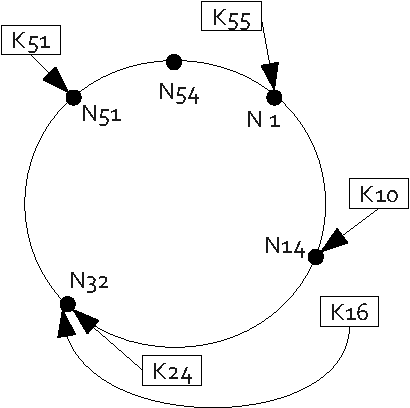
\includegraphics{grafics/chord_key_space.pdf}
\caption{Schlüsselraum ($l=6$) für Chord mit sechs Knoten ($Nx$) und fünf Daten ($Kx$). Die gestrichelten Pfeile stellen die Einträge der Fingertabelle für Knoten $N1$ dar.}
\label{fig:chord_key_space}
\end{figure}


\paragraph{Pastry / Tapestry}
Pastry \cite{Rowstron2001} und Tapestry \cite{Zhao2001Tapestry,Zhao2004Tapestry} sind sich sehr ähnlich, da beide auf Plaxtons Arbeit \cite{Plaxton1997Accessing} aufbauen. Auf Unterschiede wird explizit hingewiesen.

Pastry besitzt ebenfalls einen l-bit wertigen Schlüsselraum, dabei werden Schlüssel als Zahlen zur Basis $2^b$ dargestellt\footnote{l meist 128; b meist 4}, wobei die Wahl von $b$ einen Einfluss auf das Routing hat. Ein Datum ist dem Knoten zugewiesen, dessen ID den kleinesten Abstand zum Schlüsselwert des Datums hat.\\
\Fref{fig:pastry_key_space} zeigt dies beispielhaft für die gleichen sechs Knoten und fünf Datensätzen wie in \Fref[plain]{fig:chord_key_space}. Im Unterschied zu Chord ist jedoch Knoten $N14$ für $K16$ und Knoten $N54$ für $K55$ zuständig.

Tapestry erzeugt automatische Redundanz, da dessen Algorithmus die Daten automatisch auf mehrere Knoten verteilt.

\begin{figure}[htbp]
\centering
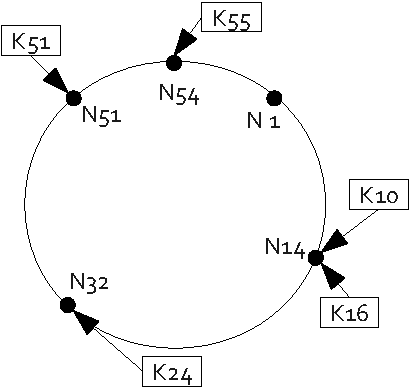
\includegraphics{grafics/pastry_key_space.pdf}
\caption{Schlüsselraum ($l=4$) für Pastry mit sechs Knoten ($Nx$) und fünf Daten ($Kx$).}
\label{fig:pastry_key_space}
\end{figure}


\paragraph{CAN}
Der Schlüsselraum bei CAN \cite{Ratnasamy2001Scalable} ist ein d-dimensionaler Torus. Die Schlüssel werden als d-Tupel (zum Beispiel $(x,y)$ für $d=2$) dargestellt. Wie bei Pastry ist der numerisch nächst gelegene Knoten für ein Datum zuständig. Der Schlüsselraum ist in nicht überlappende Zonen eingeteilt und hat eine feste Größe. Jeder Knoten \emph{besitzt} eine solche Zone, über deren Ausmaß er definiert ist. Er ist für alle Daten zuständig, deren Schlüssel in dieser Zone liegt. Ein Schlüssel wird wie bei \ac{dht} üblich über eine segmentierte Hashfunktion berechnet. Jedes Segment bildet dabei eine Dimension ab.

\Fref{fig:can_key_space} zeigt einen zweidimensionalen Schlüsselraum mit den drei Knoten A,B und C und fünf Daten. Der Schlüsselraum ist komplett auf die drei Knoten aufgeteilt, wobei A für den Bereich $(0, .5)-(1, 1)$, B für $(0, 0)-(.5, .5)$ und C für $(.5, 0)-(1, .5)$ zuständig ist.

\begin{figure}[htbp]
\centering
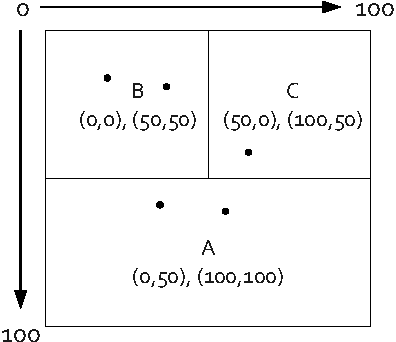
\includegraphics{grafics/can_key_space.pdf}
\caption{2-dimensionaler Schlüsselraum für CAN mit drei Knoten (A, B, C) und fünf Daten (schwarze Punkte).}
\label{fig:can_key_space}
\end{figure}


\subsection*{Routing}
\paragraph{Chord}
Bei Chord besitzt jeder Knoten eine Verbindung zu seinem direkten Vorgänger und seinem direkten Nachfolger. Eine Nachricht wird an den Nachfolger geschickt, bis sie zum zuständigen Knoten gelangt. Bei einer \emph{LOOKUP(x)}-Nachricht\footnote{Suche für key x Knoten N, so dass gilt: $N = SUCC(x)$.} prüft jeder involvierte Knoten A, ob sein Nachfolger für den Schlüssel zuständig ist, d.h. $ID_A < x \le SUCC(A)$. Ist dies der Fall, so sendet Knoten A die Antwort SUCC(A) rückwärts den Pfad der Nachricht zurück. Bei normalem Nachrichtenaustausch wird die Nachricht an den entsprechenden Knoten weitergeleitet.

Da dies eine sehr ineffizientes  Routing darstellt, pflegt jeder Knoten eine sogenannte \emph{finger table}. Die maximal $l$ Einträge in dieser Tabelle zeigen auf andere Knoten im Ring, so dass der Eintrag in Zeile $i$ von Knoten $n$ denjenigen Knoten enthält der $n$ mit mindestens $2^{i-1}$ folgt.\\
\Fref{fig:chord_key_space} stellt die Fingertabelle von Knoten $N1$ dar. Die ersten Einträge SUCC(2), SUCC(3) und SUCC(5) verweisen auf Knoten $N5$. Der dritte Eintrag verweist auf $SUCC(9) = N14$. Analog dazu ergeben sich die restlichen Einträge.

Über diese Fingertabelle können Nachrichten eine weitere Strecke auf dem Ring überbrücken und die Routingzeit wird stark verkürzt. Da die IDs in der Tabelle exponentiell zur Basis zwei ansteigen, halbiert sich die Distanz zum Ziel. Damit besitzt das Routing eine Komplexität von $O(log N)$.

\paragraph{Pastry / Tapestry}
Jeder Knoten verwaltet neben den ihm zugeteilten Daten drei Strukturen die dem Routing dienen. Diese sind das \emph{leaf set} mit Einträgen zu Knoten die im Schlüsselraum benachbart sind, das \emph{neighborhood set} mit Einträgen zu Knoten die aus Netzwerksicht nahe liegen und die Routingtabelle selbst.

\begin{figure}[htbp]
\centering
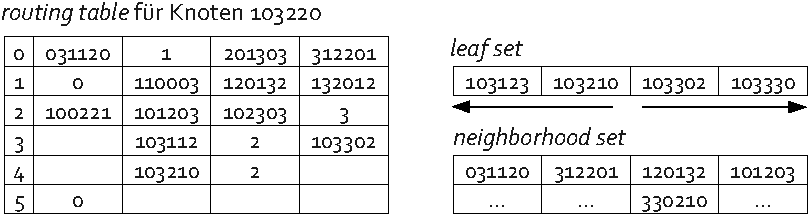
\includegraphics{grafics/pastry_routing_table.pdf}
\caption{Routing table, leaf set und neighborhood set (nach \cite{Goetz2005}) des Knoten 103220 für $l=12, b=2$. Einträge in Zeile $i$ haben einen Präfix der Länge $i$ mit dem Knoten $103220$ gemein.}
\label{fig:pastry_routing_table}
\end{figure}

Die Routingtabelle besteht aus $\frac{l}{b}$ Reihen mit je $2^b -1$ Einträgen. \Fref{fig:pastry_routing_table} zeigt dies beispielhaft für Knoten $103220$ mit $l=12, b=2$. Einträge in Zeile $i$ haben einen Präfix der Länge $i$ mit dem Knoten $103220$ gemein. Die Übereinstimmungen sind in der Abbildung fett hervorgehoben. Ist kein passender Knoten bekannt, wird das entsprechende Feld nicht ausgefüllt. Damit hat die Routingtabelle Ähnlichkeiten zur Fingertabelle bei Chord. Ein Knoten hat ungenaues Wissen über entfernte Knoten. Der Detailgrad an Routinginformationen erhöht sich pro Zeile in der Routingtabelle. Wenn im System nur sehr wenig Knoten vorhanden sind, dann sind die letzten Reihen der Routingtabelle ebenfalls nur spärlich belegt. Im Durchschnitt sind bei $n$ Knoten im System nur $log_{2^b} n$ Einträge belegt.\\
Bei der Belegung der Routingtabelle werden bei gleichem Präfix diejenigen Knoten gewählt, die aus Netzwerksicht näher sind.

Das leaf set enthält die $l$ numerisch nahen Knoten, $\frac{l}{2}$ davon sind kleiner und $\frac{l}{2}$ größer als der aktuelle Knoten. Neben Informationen zu Routingentscheidungen wird es zur Reparatur genutzt, sollten nahe gelegene Knoten ausfallen.

Das eigentlich Routing unterscheidet zwei Fälle: Zuerst prüft der Knoten ob der Schlüssel $k$ im Bereich seines leaf set ist. Ist dies der Fall, wird die Nachricht an den entsprechenden Knoten gesendet. Ist dieser Knoten für den Schlüssel zuständig, endet das Routing. Fällt $k$ nicht in den Bereich des leaf set, wird die Nachricht via Routingtabelle an einen entfernteren Knoten gesendet. Hierzu wird ein Eintrag gewählt, der eine größere beziehungsweise die größte Prefixübereinstimmung mit $k$ hat. Existiert kein solcher Eintrag, wird die Nachricht an den numerisch nächsten Knoten (zu $k$) mit gleicher Präfixübereinstimmung geschickt.\\
Da Nachrichten immer an Knoten mit einer größeren Übereinstimmung oder an nähere Knoten mit gleicher Präfixübereinstimmung gesendet werden, können keine Zyklen auftreten.

Dadurch verringert sich die Anzahl der Knoten mit längeren Präfixübereinstimmungen in jedem Schritt um mindestens den Faktor $2^b$. Somit hat das Routing eine Komplexität von $O(log_{2^b} N)$.

Das Routing von Tapestry ist sehr ähnlich zu dem hier vorgestellten Routing, allerdings nutzt Tapestry ein suffix-basiertes System. Ebenso speichert Tapestry in einem Eintrag der Routingtabelle mehrer mögliche Peers. So kann bei einem Ausfall schneller ein Ersatz gefunden werden.

\paragraph{CAN} 
Die gespeicherte Routinginformation ist bei CAN am Geringsten: Jeder Knoten speichert lediglich seine Nachbarn, das sind Knoten deren Zonen angrenzend sind, ab. Über die Zoneninformation jedes Nachbarn wird nun das Routing bestimmt. Eine Nachricht wird über den Knoten geschickt, der aufgrund seiner Zoneninformation näher am Ziel ist.

In \Fref{fig:can_routing} hat Knoten N1 die vier Knoten N2, N3, N4 und N5 als Nachbarn. Knoten N4 hingegen ist nur mit N1 und N5 benachbart.\\
Beim Routing könnte Applikationswissen genutzt werden; beispielsweise bietet Knoten N2 eine größere Bandbreite als N5 und wird deshalb zum Routen der Nachricht von N1 genutzt. 

\begin{figure}[htbp]
\centering
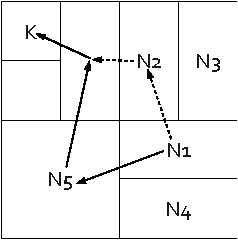
\includegraphics{grafics/can_routing.pdf}
\caption{Routing und Nachbarschaft bei CAN. Nachbarschaft von $N1 = \{N2, N3, N4, N5\}$ Routing der Nachricht von $N1$ zu $K$ via $N5$. Eine alternative Route via $N2$ ist gestrichelt dargestellt.}
\label{fig:can_routing}
\end{figure}

Die durchschnittliche Länge eines Pfades bei $d$ Dimensionen und $n$ Knoten ist $O(d\cdot n^\frac{1}{d})$. Sind die Zonen gleich aufgeteilt, so besitzt jeder Knoten max. $2d$ Nachbarn und die Anzahl an Hops verringert sich auf $O(\frac{4}{d}\cdot n^\frac{1}{d})$.


\subsection*{Nachbarschaft}
\paragraph{Chord}
Die Nachbarschaft ist bei Chord begrenzt. Jeder Knoten hat eine Verbindung zu seinem Vorgänger sowie Nachfolger auf dem Ring und hält Einträge in der Fingertabelle vor. In die Routingentscheidungen kann somit nicht direkt eingegriffen werden.

\paragraph{Pastry / Tapestry}
Das neighborhood set (siehe \Fref{fig:pastry_routing_table}) enthält $|m|$ Knoten die aus Netzwerksicht nahe sind. Obwohl es im Routing keine Rolle spielt kann es dazu genutzt werden in späteren Entscheidungen geeignete Knoten zu finden.\\
Da die Größe des leaf set ebenfalls wählbar ist, können hier ebenfalls vermehrt nahe Knoten platziert werden.


\paragraph{CAN}
Die Nachbarschaft von CAN wurde bereits im vorigen Abschnitt behandelt. Dank deren Einfachheit ist der Ein- und Austritt von Knoten zwar besonders einfach und tangiert nur wenige Knoten im Netz, jedoch kann auf die Nähe aus Netzwerksicht nur beim Eintritt eines Knotens bei der Wahl seiner Koordinaten Rücksicht genommen werden.

Die Erhöhung der Dimension bedingt eine größere Nachbarschaft und damit, neben einem kürzerem Routing, auch die Möglichkeit mehr Knoten nahe zu gruppieren. Zusätzlich können in CAN sogenannte \emph{Realitäten} genutzt werden. Dies sind verschiedene CAN-Netzwerke mit unterschiedlicher Hashfunktion zur Berechnung der Schlüssel. Jeder Knoten und jedes Datum ist in jedem dieser Netzwerke vertreten und besitzt einen unterschiedlichen Schlüssel pro Netzwerk. In einem System mit $r$ Realitäten muss ein Knoten demnach $r$ verschiedene Zonen und Nachbarschaften verwalten. Eine Nachricht wird bei jedem Routing Hop über die Realität verschickt, welche die kürzeste Route verspricht.


\subsection*{Eintritt und Austritt (Fehlerfall) von Knoten}
\paragraph{Chord}
Bei Chord kann die ID für einen neuen Knoten $n$ frei gewählt werden, es muss lediglich ein Knoten $b$ im System bekannt sein. n routet eine LOOKUP(n)-Nachricht via b und erfährt somit seinen Nachfolger auf dem Ring. In gleicher Weise vervollständigt $n$ seine Fingertabelle. Weiterhin teilt $n$ seinem Nachfolger mit, dass $n$ sein neuer Vorgänger ist.

Zur Stabilisierung und Vervollständigung der Routinginformationen arbeitet jeder Knoten im Ring periodisch die Funktion \emph{stabilize} ab. Jeder Knoten $a$ fragt seinen Nachfolger $n$ nach dessen Vorgänger $s$. Wenn $a != s$, so ist Knoten $s$ neu in den Ring eingetreten. $a$ informiert den neuen Knoten $s$, dass er sein Vorgänger ist und ändert selbst den eigenen Nachfolger auf $s$ ab. $s$ kennt nun den Bereich seiner Zuständigkeit $[ID_a, ID_s)[$ und kopiert diese Daten von seinem Nachfolger und weist diesen auf die Zuständigkeitsänderung hin.\\
Die Aktualisierung der Fingertabelle \emph{fix\_fingers} wird ebenfalls auf jedem Knoten periodisch angestoßen. Für einen zufällig gewählten Eintrag wird überprüft ob dieser noch aktuell ist.

Die verzögerte Aktualisierung hat keinen großen Einfluss auf die Korrektheit oder Geschwindigkeit des Routings, da Nachrichten an $a$ über die Nachfolger- beziehungsweise Vorgängerverbindungen der Knoten um $a$ weitergeleitet werden und somit lediglich ein weiterer Knoten involviert ist.\\
Bei einer LOOKUP(n)-Nachricht gibt der Vorgänger von n den jeweils richtigen Knoten zurück oder leitet diese Nachricht noch einmal an seinen Nachfolger weiter. Bei einer normalen Nachricht, die zum Nachfolger geroutet werden würde, kann dieser feststellen, dass er nicht mehr für das Datum zuständig ist und die Nachricht an seinen Vorgänger weiterleiten beziehungsweise selbst antworten, wenn die Daten noch nicht umkopiert sind. 

Dies bedeutet allerdings, dass der neue Knoten $n$ erst später von seinem Vorgänger erfährt und damit auch erst spät alle ihm zugeteilten Daten kennt und zu sich übertragen kann.

\begin{figure}[htbp]
\centering
\resizebox{\textwidth}{!}{%
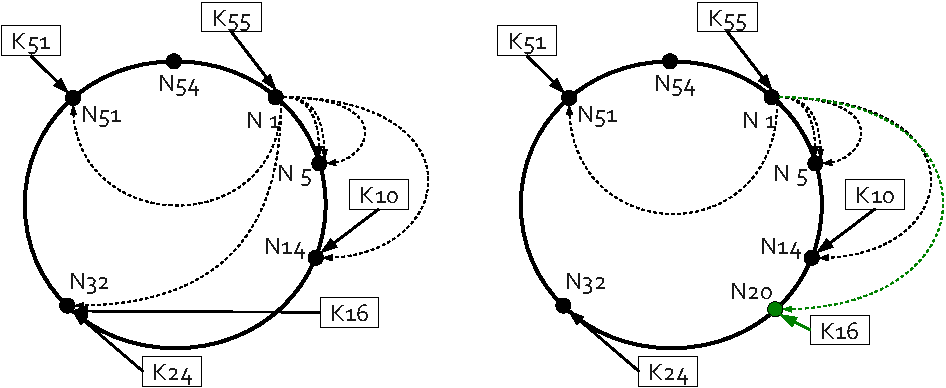
\includegraphics{grafics/chord_new_node.pdf}}
\caption{Schlüsselraum von Chord nach Ankunft von Knoten $N20$. Die Zuständigkeit für $K16$ sowie die Fingertabelle von $N1$ (gestrichelte Linien) wurden angepasst.}
\label{fig:chord_new_node}
\end{figure}

\Fref{fig:chord_new_node} verdeutlicht den Neueintritt von Knoten $N20$. Die Änderungen sind in grün dargestellt. $N1$ passt seine Fingertabelle an und $N20$ ist für $K16$ zuständig.

Der Ausfall von Knoten wird über \emph{Timeouts} ermittelt. Im Falle eines Timeouts, wird die Nachricht an den besten bekannten Vorgänger des ausgefallenen Knotens weitergeleitet. Im schlimmsten Falle ist dies der Nachfolger des sendenden Knotens. Daraus wird ersichtlich, dass ein valider Nachfolger notwendig ist. Somit hält jeder Knoten eine Liste von möglichen Nachfolgern vor, die während \emph{stabilize} erstellt werden kann. Für fehlerhafte Knoten in der Fingertabelle kann \emph{fix\_fingers} explizit aufgerufen werden.

Knotenausfall bedeutet nicht nur einen Ausfall des Knotens, sondern bedingt, dass die dort gespeicherten Daten nicht mehr erreichbar sind. Da bei Chord immer SUCC(key) für das jeweilige Datum zuständig ist, empfiehlt es sich auf Applikationsebene die Daten auf Knoten $n$ und $SUCC(n)$ zu replizieren.

Verlässt ein Knoten das Netz, so beeinflusst dies das System nicht. Jedoch ist es effizienter wenn ein verlassender Knoten seinem Vorgänger und Nachfolger dies mitteilt, die Verbindungen angepasst werden und die Daten explizit übertragen werden.

\paragraph{Pastry / Tapestry}
Einem neuen Knoten $n$ wird von Applikationsseite ein frei wählbarer Schlüssel gegeben. Meist berechnet sich dieser Schlüssel anhand dem Hashwert der IP oder seines öffentlichen Namens. Weiterhin geht das System davon aus, dass $n$ aus einer Liste bekannter Knoten denjenigen Knoten $x$ wählen kann, der aus Netzwerksicht nahe ist. Von diesem Knoten kann das neighborhood set kopiert werden. Zum Aufbau der Routingtabelle und des leaf set lässt $n$ via $x$ eine \emph{JOIN}-Nachricht an einen numerisch nahen Schlüssel zu $n$ routen. Diese Nachricht gelangt schließlich zu Knoten $c$, von dem das leaf set kopiert werden kann, da $c$ und $n$ sich nahe sind. Alle Knoten die diese \emph{JOIN}-Nachricht weiterleiten, senden ihre Routingtabelle an $n$. Für jeden Routinghop kopiert sich $n$ die entsprechende Zeile aus der Routingtabelle, da ausgehend von keiner Präfixübereinstimmung mit dem nahen Knoten $x$, jeder weitere Hop eine größere Präfixübereinstimmung bringt.\\
Im Gegensatz zur nachträglichen Aktualisierung bei Chord, wird nun die gesamte Routinginformation an alle bekannte Knoten gesendet. Der neue Knoten ist nun im Netzwerk bekannt und erreichbar.

Ausgefallene Knoten werden ebenfalls anhand von Timeouts beim Routing entdeckt. Da die Einträge des neighborhood set nicht im Routing involviert sind, müssen diese periodisch geprüft werden. Fehlerhafte Einträge in der Routingtabelle können über einen anderen Eintrag mit gleicher Präfixübereinstimmung kompensiert werden, müssen aber entfernt werden um ein stabiles und sicheres Routing zu gewährleisten. Hierzu können von benachbarten Einträgen Routinginformationen angefordert werden um die entstandene Lücke zu füllen. Ein fehlerhafter Eintrag im leaf set oder neighborhood set kann auf ähnliche Weise repariert werden: Hier werden Informationen von den anderen Einträgen im leaf set oder neighborhood set angefordert.

Der Austritt eines Knotens wird vom System wie ein Fehlerfall behandelt werden. Um die Datenintegrität zu gewährleisten und um unnötigen Nachrichtenversand im System zu vermeiden, sollte die Applikation den Austritt eines Knotens speziell behandeln.

\paragraph{CAN}
\begin{figure}[htbp]
\centering
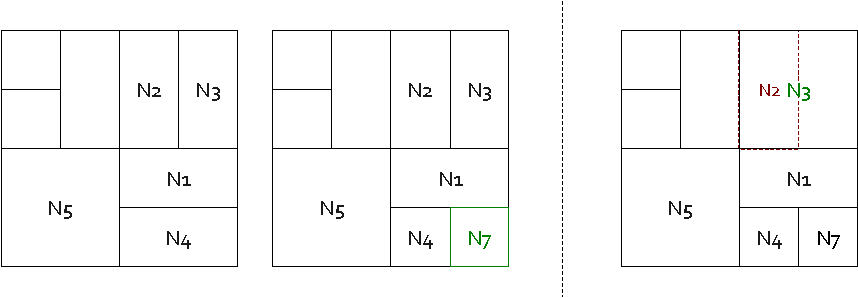
\includegraphics{grafics/can_new_node.pdf}
\caption{Eintritt und Fehlerfall bei CAN. Nach Eintritt von Knoten $N7$ und Aufteilung der Zone von $N4$ ist die Nachbarschaft von $N1 = \{N2, N3, N4, N5, N7\}$. Nach dem Ausfall von $N2$ (rot) vereinigt $N3$ die Zonen.}
\label{fig:can_new_node}
\end{figure}

Für den Eintritt eines neuen Knoten n muss wieder ein Knoten b aus dem Netz bekannt sein. Eine Koordinate im Schlüsselraum wird n zugewiesen und eine spezielle \emph{JOIN}-Nachricht via d an die gewählte Koordinate gesendet. Ist diese Nachricht über das normale Routing bei dem für diese Koordinate zuständigen Knoten d angekommen, halbiert dieser seine Zone und weist eine Hälfte dem neuen Knoten n zu. Die Aufteilung der Zonen erfolgt dabei anhand einer Reihenfolge der Dimensionen. Dies vereinfacht die Aufteilungs- sowie die Zusammenführungsprozedur. Letztlich kopiert d alle Daten aus dieser neuen Zone zu n. Knoten d schickt n seine Nachbarschaftsinformationen und trägt diesen selbst als neuen Nachbarn ein. Knoten n teilt seine Anwesenheit sofort seinen neuen Nachbarn mit. Der Neueintritt eines Knotens ist damit auf ein paar Nachrichten zwischen der Nachbarn begrenzt und beeinträchtigt das übrige Netzwerk nicht. Über periodische \emph{UPDATE}-Nachrichten halten sich Nachbarn stets aktuell und senden ihre eigene Nachbarschaftsinformationen an die benachbarten Knoten.\\
\Fref{fig:can_new_node} zeigt den Eintritt für Knoten N7. Nach Teilung der Zone von N4 verändert sich die Nachbarschaft von N1: Knoten N7 kommt neu hinzu.

Ausstehende \emph{UPDATE}-Nachrichten oder Timeouts weisen auf ausgefallene Knoten hin. Werden diese zum Routen einer Nachricht benutzt stellt dies keine direkte Beeinträchtigung des Netzes dar, da die Nachricht über einen anderen Nachbarn verschickt werden kann. So könnte N1 auch N2 zum Nachrichtenversand nutzen, wenn N5 ausgefallen wäre (vergleiche \Fref{fig:can_routing}).

Ein Knoten der einen ausfallenden Peer entdeckt hat, startet einen Timer, dessen Dauer proportional zur Zonengröße ist. Nach Ablauf sendet der Knoten eine spezielle \emph{TAKEOVER}-Nachricht an alle Nachbarn des ausgefallen Knotens\footnote{Dieses Wissen ist durch vorherige \emph{UPDATE}-Nachrichten bekannt.}. Erreicht eine \emph{TAKEOVER}-Nachricht einen Knoten, stoppt dieser seinen eigenen Timer falls seine Zone größer als die des Sender ist. Andernfalls antwortet er selbst mit seiner \emph{TAKEOVER}-Nachricht. Auf diese Weise wird der Nachbar mit der kleinsten Zone gefunden. Dieser ist nun der neue Besitzer der Zone und fügt seine beiden Zonen zusammen wie es in \Fref{fig:can_new_node} am Beispiel von N2 und N3 ersichtlich ist. N2 (rot dargestellt) ist ausgefallen und N3 vergrößert seine Zone. N2 ist nun nicht mehr in der Nachbarschaft von N1 enthalten. Es ist möglich, dass ein Knoten Besitzer zweier Zonen wird, welche sich nicht als eine Zone darstellen lassen. Ein Beispiel hierfür ist Knoten N4 der beim Ausfall von N5 dessen Zone übernimmt. Ein Hintergrundprozess defragmentiert solche Zonen und weist Knoten gegebenenfalls neue Koordinaten zu.\\
Eine periodische Auffrischung der Datensätze soll auch hier einen Verlust im Fehlerfall schnell kompensieren.

Möchte ein Knoten l das System verlassen, so sucht er einen Nachbarn mit der kleinsten Zone und sendet diesem seine Daten. Dieser Nachbar informiert nun die alten Nachbarn von l über die geänderte Nachbarschaft.

\subsection*{Tauglichkeit als Basis für Publish/Subscribe}
Publish/Subscribe-Systeme können als Anwendungsfall von \ac{cast} gesehen werden. Dies ist selbst eine Anwendung der generischen KBR-API. Alle untersuchten Netzwerke genügen dieser und sind somit als Basis für \ac{cast} nutzbar.

Für Pastry und Tapestry gibt es die Publish/Subscribe-Systeme Scribe und Bayeux die nach dem Prinzip des \emph{Multicast-Tree} aufgebaut sind \cite{Castro2002Scribe, Zhuang2001}.\\
Für CAN existiert ein System namens CAN-Multicast, welches allerdings die Nachrichten per \emph{flooding} verschickt \cite{Ratnasamy2001}.

\subsection*{Fazit}
Eine generelle Übersicht der Systeme stellt \Fref{tab:evaluation_fazit} dar. Jedes System hat eigene Schwächen und Stärken. So bezahlt CAN einen günstigen Ein- und Austritt der Knoten dank der kleinen Nachbarschaft mit mehr Routing Hops als beispielsweise Chord. Dieses hat durch seine Fingertabelle wiederum mehr Einfluss auf das Routing, aktualisiert diese Tabellen jedoch erst nachträglich im Hintergrund während dies bei Pastry aktiv geschieht.

\Fref{tab:evaluation_fazit} (Auszug aus \cite{Goetz2005}) listet die durchschnittlich anfallenden Kosten (Routing Hops, Größe der Routinginformation, Nachrichtenanzahl beim Ein- und Austritt) für die drei getesteten System auf.

\begin{table}[htbp]
\centering
\label{tab:evaluation_fazit}
\begin{tabular}{lcccc}
\toprule
 & Routing Hops & Routinginformation & Eintritt & Austritt\\ 
 \cmidrule{2-5}
Chord & $O(\frac{1}{2}log_2~n)$ & $O(2log_2~n) $ & $ O(log_2^2 n) $ & $ O(log_2^2 n) $ \\
Pastry & $O(\frac{1}{b}log_2~n)$ & $O(\frac{1}{b} (2^b-1) log_2~n) $ & $ O(log_{2^b}~n) $ & $ O(mlog_b~n) $ \\
CAN & $O(\frac{d}{2}n^\frac{1}{d})	$ & $O(2 d) $ & $ O(\frac{d}{2}n^\frac{1}{d}) $ & $ O(2 d) $ \\
\bottomrule
\end{tabular}
\caption{Vergleich der Systeme Chord, Pastry und CAN anhand einiger Gesichtspunkte. $n$ ist die Anzahl der Knoten, $b$ die Anzahl der Bits der darstellenden Basis bei Pastry und $d$ die Anzahl der Dimensionen bei CAN. (aus \cite{Goetz2005})}
\end{table}

Für uniformes Routing (d.h. das Routing ist bei allen Peers gleich) sind $O(log~n)$ beziehungsweise $O(n\frac{1}{d})$ Hops für Routingtabellen der Größe $O(log~n)$ beziehungsweise $O(d)$ die asymptotischen Grenze \cite{Xu2004Fundamental}. Die vorgestellten \ac{dht}-basierten Netzwerke nutzen ein uniformes Routing.


\paragraph{Geringe Latenz und Kommunikation über das Netzwerk}
Bei Pastry/Tapestry sind die kürzesten Routen und damit auch oftmals geringste Latenz im Nachrichtenversand zu erwarten, da die Routingtabelle im Vergleich zu Chord und CAN mehr Einträge enthält und diese einfacher mit - aus Netzwerksicht - nahen Peers belegt werden kann. Bei CAN hingegen wird das langsamste Routing erwartet, da Nachrichten nur zwischen benachbarten Knoten ausgetauscht werden. Sprünge (via Fingertabellen) sind nicht vorgesehen. Die Erwartungen decken sich mit den Werten in \Fref{tab:evaluation_fazit}.

Li stellt für verschiedene Parametereinstellungen der Netzwerke deren Bandbreite und Latenz gegenüber und untersucht dabei das Verhalten bei gehäuften Ein- und Austritten von Knoten. Hier ist Chord leicht im Vorteil, da lediglich der Verweis auf den Nachfolgeknoten für das korrekte Routing erforderlich ist. Bei allen Netzwerken pendelt sich die Latenz im \emph{worst case} auf 250ms ein \cite{Li2004Comparing}.

Die Vorteile der Kommunikation bei Pastry/Tapestry überwiegen für unseren Anwendungsfall.

\paragraph{Skalierbarkeit}
CAN steht hier an erster Stelle, da Ein- und Austritte von Peers nur wenige Knoten im Netz betreffen. Auch bei vielen Ein- und Austritten leidet das Netz unter keiner großen Nachrichtenlast. Allerdings leidet die Kommunikation in großen Netzen (siehe obigen Punkt). Chord liegt auf dem letzten Platz, da das Netzwerk erst durch später aufgerufene Methoden vollkommen funktionsfähig wird (siehe \emph{Eintritt und Austritt (Fehlerfall) von Knoten}).

Hier stellt sich nun die Frage, warum ein neuer Knoten $n$ nicht beim Eintritt seinen Nachfolger $p$ nach dessen altem Vorgänger befragt und somit die Zuständigkeit der Daten gleich beim Eintritt klärt?\\
Eine mögliche Antwort ist, dass dadurch eine Mehrbelastung durch das Umkopieren von Daten entstehen, ohne dass dadurch das Routing beziehungsweise Auffinden der Daten merklich verbessert würde. Im Falle von häufigen Eintritt und Austritt von Knoten würde das Netz lahm gelegt. Pastry und Tapestry liegen auf Zweitem Platz; der Aufbau der Routingtabelle erfolgt in vielen kleinen Schritten - dafür ist ein Knoten danach ein vollwertiger Peer im System.

\paragraph{Fehlertoleranz bei Knotenausfall}
Alle Systeme finden ausgefallene Knoten durch periodisch versandte Nachrichten an benachbarte Peers oder durch Timeouts verschickter Nachrichten. Jedes System kompensiert solch einen Fall auf eigene Art und Weise. Bei CAN wird ein Knoten seine mit der verlassenen Zone verbinden, Knoten in Chord aktualisieren ihre Fingertabellen und Peers in Pastry und Tapestry versuchen durch Befragungen anderer Knoten die entstandene Lücke in der Routingtabelle zu füllen. Ein Knotenausfall hat bei CAN allerdings die geringsten Auswirkungen auf das restliche System, da nur die Nachbarknoten involviert sind. Dies ist der kleinen Routingtabelle geschuldet.

Alle Systeme fordern jedoch die Applikation zu einer periodischen Auffrischung der gespeicherten Daten auf und bieten selbst kaum Redundanz (Ausnahme Tapestry) an.


\paragraph{Bestimmung der Nachbarschaft}
Allein die Größe der Routingtabelle bedingt, dass bei Pastry und Tapestry mehr Einfluss auf die Zusammenstellung genommen werden kann. Bei CAN gibt es faktisch nur eine Entscheidung bei Eintritt in das Netz, Chord bietet über die Fingertabelle minimalen Einfluss, während bei Pastry explizit das Neighborhood Set eingesetzt wird, um eventuelle Lücken in der Routingtabelle geschickt zu besetzen.

\paragraph{Eingriff in Routingentscheidungen}
Das Routing bei CAN kann nur bedingt beeinflusst werden: An welchen Nachbarn soll die Nachricht geschickt werden. Chord hingegen bietet mit seiner Fingertabelle mehr Variationsmöglichkeiten - allerdings nur für die zu überbrückende Distanz im Schlüsselraum. Pastry und Tapestry verbinden diese Variationen mit vielfältigen Nachbarschaftsoptionen.

\paragraph{Unterbau für \ac{cast}}
Die Implementierung von Scribe und Bayeux für Pastry und Tapestry zeigen, dass diese als Unterbau für \ac{cast} sehr wohl geeignet sind. Aufgrund der mageren Ergebnisse in Castros Untersuchung \cite{Castro2003Evaluation} bleibt CAN trotz interessanter Ideen außen vor. Ebenso kann Chord nicht in Betracht gezogen werden, da es kurzzeitige Inkonsistenzen in der Nachbarschaft (und damit dem Routing) geben kann. Weiterhin wird eine größere Latenz im Nachrichtenversand erwartet, da Nachrichten nur in einer Richtung auf dem Ring weitergeleitet werden.

\subsection*{Auswahl des Netzwerkes}
Die Konzeption des Netzes ist ausschlaggebender als Implementierungsdetails. Die Evaluation zeigt, dass ein Netzwerkaufbau wie bei Pastry/Tapestry  ein möglicher Kandidat ist.\\
Pastry ist als Javabibliothek\footnote{\url{http://www.freepastry.org}} verfügbar und die Entwicklung von Tapestry (ebenfalls in Java implementiert) wurde mit Version 2.01 eingestellt. Chimera \cite{Allen2006Chimera} ist der Nachfolger von Tapestry und vereint das Beste von Pastry und Tapestry in sich\footnote{siehe \url{http://current.cs.ucsb.edu/projects/chimera/index.html}}: 
\begin{quote}
Chimera is a light-weight C implementation of a ``next-generation'' structured overlay that provides similar functionality as prefix-routing protocols Tapestry and Pastry.  Chimera gains simplicity and robustness from its use of Pastry's leafsets, and efficient routing from Tapestry's locality algorithms.  In addition to these properties, Chimera also provides efficient detection of node and network failures, and reroutes messages around them to maintain connectivity and throughput.  
\end{quote}

Der frei verfügbare Code (veröffentlicht unter GPL), die Anpassbarkeit und die Unterstützung der Zielplattformen Linux und Windows sprechen für Chimera. Weiterhin entspricht Chimera der generischen \ac{api} und kann bei gravierenden Problemen durch ein anderes System ausgetauscht werden, ohne das restliche System zu beeinflussen.

In diesem Kapitel wurden die drei Netzwerke Chord, Pastry/Tapestry und CAN verglichen und ihre unterschiedlichen Arbeitsweisen erklärt. Es zeigt sich, dass das Konzept von Pastry/Trapestry für \ac{m2etis} gut geeignet ist. Damit ist der erste Teil dieser Arbeit, die Auswahl eines geeigneten Netzwerkes, abgeschlossen. Das nächste Kapitel befasst sich nun mit der Konzeption des Frameworks, das auf dem Netzwerk aufsetzt.
